\section{Beam Direct Stiffness Method}

A beam element has four degrees of freedom. Two degrees of freedom at each node which includes the rotation, $\theta$, and the deflection or transverse displacement, $w$.

\begin{figure}[h]	
	\centerline{
		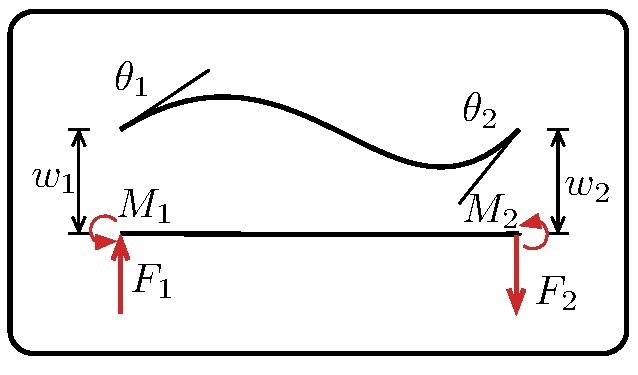
\includegraphics[width=0.7\columnwidth]{Figures/DeflectionandRotation}
		}
	\caption{Degrees of Freedom}
	\label{fig:DeflectionandRotation}
\end{figure}

\subsection{Bending Stiffness}

We will isolate each degree of freedom by applying boundary conditions at each node, such that each beam will only have one unrestrained kinematic unknown. Figures \ref{Fig:BeamIso1} and \ref{Fig:BeamIso2} show the various boundary conditions that will be used to determine the beam bending stiffness. This will allow us to derive the force-displacement relationship necessary to solve the beam.

%\begin{figure}[H]
%	\centerline{
%		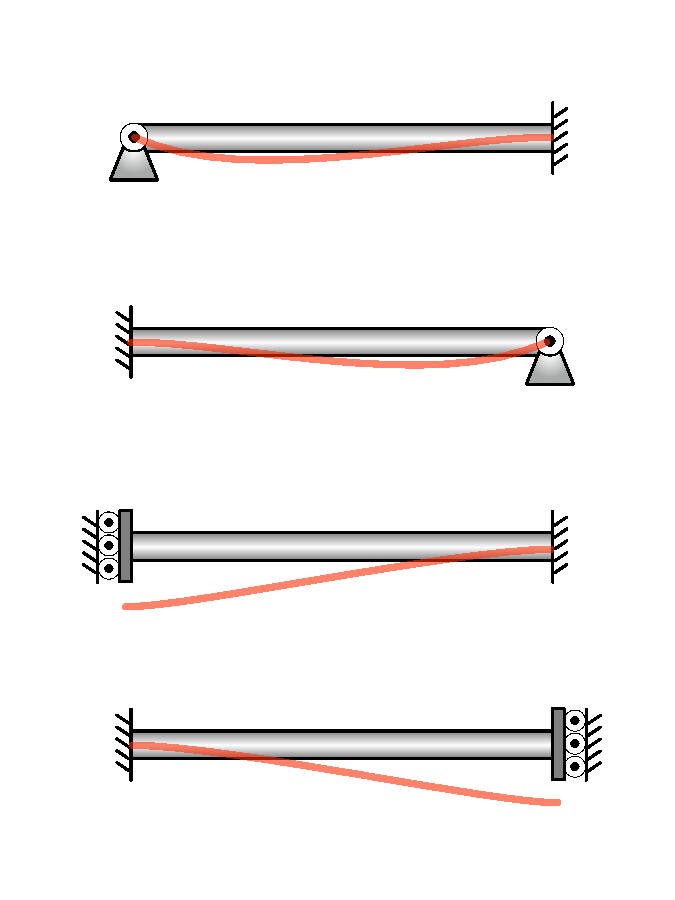
\includegraphics[width=0.8\columnwidth]{Figures/BCFrame}
%		}
%	\caption{Beam Boundary Conditions}
%	\label{fig:BCFrame}
%\end{figure}

\begin{figure}[h]
\begin{center}
\begin{tikzpicture}
	
	\point{A}{0}{0}
	\point{B}{5}{0}
	\beam{4}{A}{B}
	\support{3}{A}[-90]
	\support{4}{B}[90]
	
	\draw[red, thick, dashed] (0,0) .. controls (3,0) and (3,-1) .. (5,-1);
	
	\point{A}{0}{-2}
	\point{B}{5}{-2}
	\beam{4}{A}{B}
	\support{4}{A}[-90]
	\support{3}{B}[90]

	\draw[red, thick, dashed] (0,-3) .. controls (2,-3) and (2,-3) .. (5,-2);


\end{tikzpicture}
\caption{Isolation of Deflection}
\label{Fig:BeamIso1}
\end{center}
\end{figure}

\begin{figure}[h]
\begin{center}
\begin{tikzpicture}
	
	\point{A}{0}{0}
	\point{B}{5}{0}
	\beam{4}{A}{B}
	\support{3}{A}[-90]
	\support{1}{B}[0]
	
	\draw[red, thick, dashed] (0,0) .. controls (3,0) and (3,-1) .. (5,0);
	
	
	\point{A}{0}{-2}
	\point{B}{5}{-2}
	\beam{4}{A}{B}
	\support{1}{A}[0]
	\support{3}{B}[90]
	
	\begin{scope}[yscale=1,xscale=-1,xshift=-5cm]
	\draw[red, thick, dashed] (0,-2) .. controls (3,-2) and (3,-3) .. (5,-2);
	\end{scope}
	
\end{tikzpicture}
\caption{Isolation of Rotation}
\label{Fig:BeamIso2}
\end{center}
\end{figure}


\begin{align*}
	w_0=0 & \text{	} \theta_0=?\\
	w_L=0 &\text{	}  \theta_L=0
\end{align*}

The following variables will be used for notational convenience when defining the beam stiffness matrix.

\begin{center}
	\begin{tabular}{cccc}
		$a=\frac{12EI}{L^3}$ & $b=\frac{6EI}{L^2}$ & $c=\frac{4EI}{L}$ & $d=\frac{2EI}{L}$
	\end{tabular}
\end{center}

The local element stiffness matrix for a beam is therefore:
\begin{align}
	\begin{Bmatrix}
		V_0\\ M_0\\ \hline V_L\\ M_L
	\end{Bmatrix}
	=
  \underbrace{
	\left[
	\begin{array}{cc|cc}
		a & b & -a & b\\
		b & c & -b & d\\ \hline
		-a & -b & a & -b\\
		b & d & -b & c
	\end{array}
	\right]
  }_{\vec{k_{local}}}
	\begin{Bmatrix}
		w_0\\ \theta_0\\ \hline w_L\\ \theta_L
	\end{Bmatrix}
\end{align}

The global element stiffness matrix will not be discussed since a beam only has elements along one coordinate system. 